\subsection{Communication}
\label{subsec:communication-software}

Communication between the door nodes and control server using ThingSpeak is one
of the key challenges of this project. Several class will be written in order to
provide a reliable transport layer on top of ThingSpeak and to convey our
application information between endpoints. A class diagram of our communications
classes is shown in figure \ref{fig:communication-classes}

\begin{figure}[!htb]
\centering
\includegraphics[width=\textwidth]{uml/communication-classes.png}
\caption{UML Class Diagram of Communications Classes}
\label{fig:communication-classes}
\end{figure}

Our Channel class represents a ThingSpeak channel. This class will make use of
the requests library in order to provide methods that allow data to be read
from and written to a ThingSpeak channel.

The Connection class acts like a socket that makes use of a ThingSpeak channel
for communication. A ThingSpeakPoller thread is used by the channel class to
check for new messages on the ThingSpeak channel.

The Server class is used to listen for new connections. On the server side, a
Server class instance is created which will instantiate a new Connection object
whenever a client connections to it. On the client side the Connection
constructor is used directly to create a connection to a server that is already
running on another endpoint. Once both sides have a Connection object they are
free to send messages to each other over the ThingSpeak channel.

The application layer message format (as described in section
\ref{subsec:communication-protocol}) is implemented by the series of classes
shown in figure \ref{fig:message-classes}.

\begin{figure}[!htb]
\centering
\includegraphics[width=\textwidth]{uml/message-classes.png}
\caption{UML Class Diagram of Application Layer Message Classes}
\label{fig:message-classes}
\end{figure}

The message classes encapsulate all of the marshalling and unmarshalling
functionality.

\subsection{Door Node}

The door node code consists of classes which abstract over the interface to each
of the hardware devices at the door node and a singleton control class that
encapsulates the control logic. The class structure of the door node is shown in
figure \ref{fig:door-node-classes}.

\begin{figure}[!htb]
\centering
\includegraphics[width=\textwidth]{uml/door-node-classes.png}
\caption{UML Class Diagram for Door Node Software}
\label{fig:door-node-classes}
\end{figure}

As well as instances of the hardware abstraction classes, the DoorNodeController
class has an instance of the Channel class and an instance of the Connection
class, as described in section \ref{subsec:communication-software}. These
objects are used to facilitate communication with the control server.

The logic employed by the door node is shown in figure
\ref{fig:door-node-logic}.

\begin{figure}[!htb]
\centering
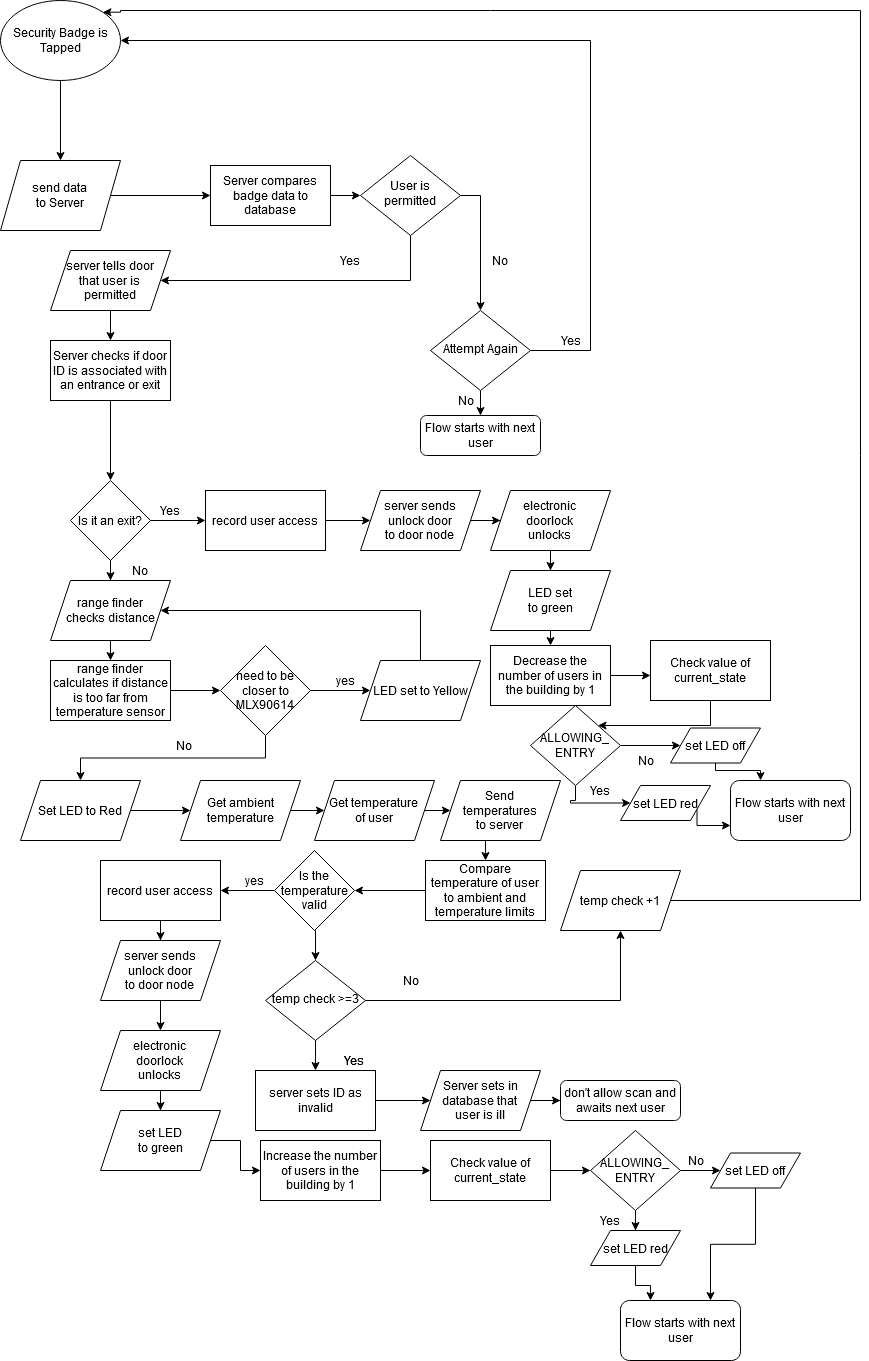
\includegraphics[width=0.75\textwidth]{images/door-node-flow.png}
\caption{Door Node Control Logic}
\label{fig:door-node-logic}
\end{figure}

\subsection{Control Server}

The control server code consists of a class that abstracts over the database
operations, a singleton class that encapsulates the control server logic, and a
GUI class. The class structure of the control server is shown in figure
\ref{fig:control-server-classes}.

\begin{figure}[!htb]
\centering
\includegraphics[width=0.6\textwidth]{uml/control-server-classes.png}
\caption{UML Diagram of Control Server Classes}
\label{fig:control-server-classes}
\end{figure}

The ServerController class has an instance of the Channel class, an instance
of the Server class and potentially multiple instances of the Connection class
described in section \ref{subsec:communication-software}. These objects are used
to facilitate communication between the control server and door nodes.

The ServerController also has an instance of the OperatorGUI.  The settings
object in the OperatorGUI is queried each time an access request is made to
determine access permissions.  The Operator can use the GUI the change and save
the settings.  The Operator can also use the GUI to perform queries on the
database.
